
\section{Safety and Robustness in Quantized Neural Networks}

Neural Networks have begun to replace work previously performed by human professionals. For example, in pattern recognition, computers perform tasks similar to those of doctors. Unlike humans, a computer can process large numbers of images and classify them with high accuracy. However, new adversarial attack techniques have made the use of machine learning more challenging. Techniques such as Fast Gradient Sign Method (FGSM) \& R+FGSM \cite{goodfellowExplainingHarnessingAdversarial2015}, Random Perturbation, and Basic Interactive Method \cite{kurakin2017adversarialmachinelearningscale} allow an attacker to subtly alter the input data. These small perturbations, although imperceptible to humans, are specifically designed to cause the model to misclassify the input as defined in Definition \ref{definition:adversarial_attack} \cite{goodfellowExplainingHarnessingAdversarial2015}.
\newpage
\begin{figure}
    \centering
    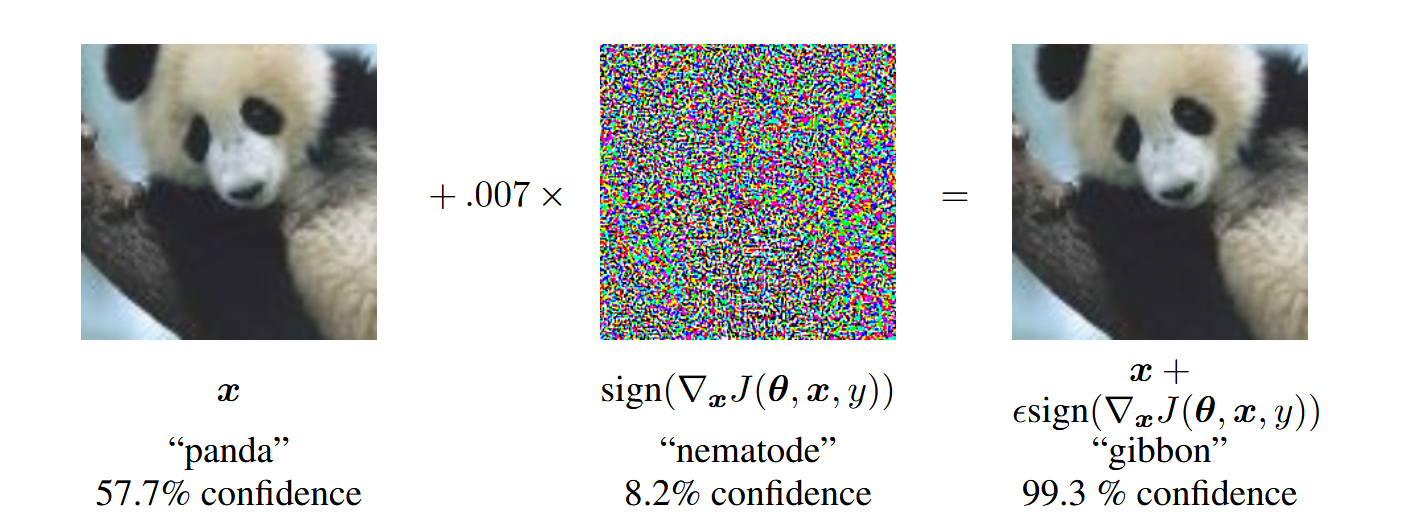
\includegraphics[width=1\textwidth]{figuras/2-fundamentos/safety/adversarial_attack_panda_example.png}
    \caption{Adversarial Attack Extracted from \cite{goodfellowExplainingHarnessingAdversarial2015}}
    \label{fig:panda_example_safety}
    \end{figure}
    
ANNs and QNNs are like black boxes: in practice, we only control the input and observe the output, while the internal reasoning is not explicitly accessible. As a result, most safety and security properties naturally express as constraints on their input-output relations. To formalize this, let $f$ be the network function mapping an input $x \in \mathcal{I}$ to an output space $\mathcal{O}$. Then, a generic safety requirement can be stated as: for every input $x \in \mathcal{I}$, the produced output must lie in a desired set $\mathcal{G}$, i.e., it must satisfy the property $P$:
\[
\forall x \in \mathcal{I} \;\Rightarrow\; f(x) \in \mathcal{G}.
\]

Building on this formal framework, one important safety-related property is adversarial robustness. This property is usually regarded as the requirement that small perturbations in the input should not change the model decision. The predicted label must stay the same even if the input is slightly modified \cite{huangSurveySafetyTrustworthiness2020, linIntegerarithmeticonlyCertifiedRobustness2021}. Consider an input domain $\mathcal{D}$ and a neighborhood around a specific input $x \in \mathcal{D}$, defined by a metric $d_{\text{in}}$ and referred to as $\mathcal{I}(x,d_{\text{in}})$. If $y$ represents the correct label for $x$, robustness can be formalized as:
\[
\forall  x' \in \mathcal{I}(x,d_{\text{in}}) \;\Rightarrow\; f(x') = y.
\] 

Here, $\mathcal{I}(x,d_{\text{in}})$ is typically constrained by a radius $\epsilon$. This means the distance between two values must be less than or equal to $\epsilon$, for example, $d_{\text{in}}(x,x') \le \epsilon$ \cite{huangSurveySafetyTrustworthiness2020}. This research uses an $L_\infty$ ball, which restricts the maximum deviation for each feature:
\[
\mathcal{I}(x,\epsilon) = \left\{ x' \in \mathbb{R}^n \;\middle|\; \|x - x'\|_\infty \le \epsilon \right\}.
\]

As defined in the survey \cite{huangSurveySafetyTrustworthiness2020}, the adversarial attack can be defined as in Definition \ref{definition:adversarial_attack}.

\begin{definition}[Adversarial Example]\label{definition:adversarial_attack}
Given an ANN $f : \mathcal{I} \to \mathcal{O}$, a human decision oracle $\mathcal{H} : \mathcal I \to \mathcal{O}$, and a legitimate input $x \in \mathcal{I}$ with $\arg \max_j f_j(x) = \arg \max_j \mathcal{H}_j(x)$, an adversarial example to an ANN is defined as:
\begin{equation}
\begin{aligned}
\exists \hat{x} : \quad & \arg \max_j \mathcal{H}_j(\hat{x}) = \arg \max_j \mathcal{H}_j(x) \\
& \wedge ||x - \hat{x}||_p \leq d \\
& \wedge \arg \max_j f_j(\hat{x}) \neq \arg \max_j f_j(x)
\end{aligned}
\end{equation}
where $p \in \mathbb{N}, p \geq 1, d \in \mathbb{R}$, and $d > 0$.
\end{definition}

The cause of vulnerability to \textit{adversarial examples} is likely due to the extreme nonlinearity of Neural Network Models \cite{goodfellowExplainingHarnessingAdversarial2015}. Even small errors may lead to misclassification of the Neural Network due to the "error amplification effect," in which small residual adversarial noise is progressively amplified through the network's layers \cite{liaoDefenseAdversarialAttacks2018}.  

\subsection*{Quantization and Robustness}
As discussed previously, Quantization introduces statistical errors into the Quantized model. These errors may affect the model's ability to classify and operate properly on input data. Thus, there is a need to assess safety features. Quantization amplifies the perturbation, i.e., it makes the model more sensitive to input perturbations \cite{zhangQEBVerifQuantizationError2023}, thereby leading the new model to misclassify more frequently than the baseline one. It inherently makes the model more susceptible to adversarial attacks. As explained by Sena et al. in \cite{sena2021verifying}, due to lower bit-width, even small perturbations can significantly alter hidden-layer activations, leading the model to misclassify.

Additionally, quantization affects decision boundaries \cite{gorslineAdversarialRobustnessQuantized2021}. During weight reduction, the network loses the ability to define smooth boundaries and thus to perform precise class inference. This directly influences gradient-based attacks, because the attacker aims to hit the region where misclassification occurs \cite{gorslineAdversarialRobustnessQuantized2021}.

In the work of \cite{goodfellowExplainingHarnessingAdversarial2015}, it's shown that the accuracy drop happens later than the adversarial vulnerability: It states that with quantization, the accuracy of the model in the work does not drop until a 4-bit bit-width is chosen, though the drop happens with 5 bit-width when attacked by the adversarial attack, dropping by 25\% the accuracy of the model.

Further supporting the need for careful analysis, a concept defined by Giacobbe et al. in \cite{giacobbe2020how} proves that robustness is not non-monotonic bitwise, i.e., a 32-bit model may become vulnerable if quantized to 8-bit precision, but another model might as well become vulnerable if the precision is increased, e.g., from 6 to 8. This phenomenon underscores the need for bit-precision verification, as anything can happen to a model when bit precision is swapped.

